% ----------------------------------------------------------------------
% Date: September 23th, 2016
% Author: Roberto Metere
% Project: Beamer template for Newcastle University
%
% Copyright (C) 2016-2018 Roberto Metere
% ----------------------------------------------------------------------
%
\documentclass[t,compress,9pt,aspectratio=169]{beamer}
\usepackage[english]{babel}
\usepackage[utf8]{inputenc}
\usepackage[nclbghead]{nclbeamer}
\usepackage{listings}
\usepackage[UKenglish, nodayofweek]{datetime}


\usepackage{natbib}

\setcitestyle{notesep={: }}
\setlength{\bibsep}{6pt plus 0.5ex}

\usepackage{hyperref}
\hypersetup{
    colorlinks=true,
    linkcolor=nclblue,
    citecolor=nclblue,
    filecolor=magenta,      
    urlcolor=nclblue,
    pdftitle={Overleaf Example},
    pdfpagemode=FullScreen}

% Set to 1 or comment to disable transparency and enable full opacity.
\setblockbodyopacity{0.5}

% Listings
\definecolor{cident}{rgb}{0,0.33,0.42}
\definecolor{ckeyw}{rgb}{0,0,0.8}
\definecolor{ccomm}{rgb}{0,0.8,0}
\definecolor{cstr}{rgb}{0.8,0,0}

\lstset{language=[LaTeX]{TeX},
  basicstyle=\footnotesize\ttfamily,
  keywordstyle=\color{ckeyw}\bfseries,
  identifierstyle=\color{cident}\bfseries,
  commentstyle=\color{ccomm},
  stringstyle=\color{cstr},
  showstringspaces=false,
  breaklines=true,
  breakatwhitespace=true,
  tabsize=2,
%   numbers=left,
%   stepnumber=1,
%   firstnumber=1,
%   numberfirstline=true,
  }
  
  
  
  
  

%%%%%%%%%%%%%%%%%%%%%%%%%%%%%%%%%%%%%%%%%%%%%
% Document Information
%%%%%%%%%%%%%%%%%%%%%%%%%%%%%%%%%%%%%%%%%%%%%
\nclsetidentity{School of}{Geography, Politics and Sociology}
\title[Shorttitle]{\textbf{Example presentation title here}}
\subtitle{Subtitle}
\author[Shortauthor]{Author \\ \small email: \href{mailto:author@ncl.ac.uk}{author@ncl.ac.uk}}
\institute{Newcastle University}
\date{\today}



% \setlength{\frametitlemargin}{1mm}
\begin{document}
% ==============================================================
%                         --- Welcome frame
% ==============================================================
\begin{frame}[plain]
\maketitle
\end{frame}



% ==============================================================
%                         --- TOC
% ==============================================================
\begin{frame}
\frametitle{Overview}
\tableofcontents
\end{frame}



% ==============================================================
%                         --- Section 1
% ==============================================================
\section{1.0 Introduction}
\begin{frame}[fragile]
  \frametitle{Introduction}
    \begin{itemize}
      \item \textbf{List of things}
      \item \textbf{And more things}
        \begin{itemize}
      	       \item This is an example of a nested list
      	       \item This is an example of a nested list
      	\end{itemize}
      \item \textbf{Key Skills}
          \begin{itemize}
      	      \item Writing lists
      	      \item This is an example of a nested list
      	      \item This is an example of a nested list
          \end{itemize}
    \end{itemize}
\end{frame}




% ==============================================================
%                         --- Section 2
% ==============================================================
\section{2.0 Theory}
\begin{frame}[fragile]
  \frametitle{Split frame in two}
  
    \begin{columns}[T] % align columns
      \begin{column}{.45\textwidth}
        \textbf{Left Part}
            \begin{itemize}
              \item{List of things}
              \item{And more things}
          \end{itemize}
      \end{column}%
      
      \hfill%
      \begin{column}{.45\textwidth}
        \textbf{Right Part} \\
        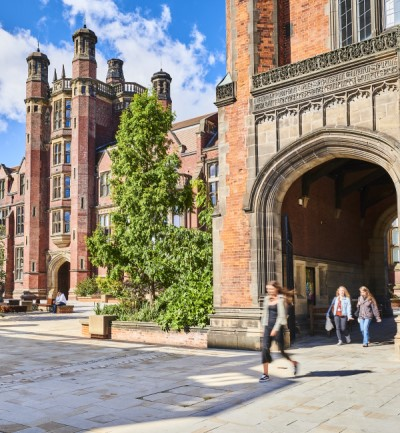
\includegraphics[scale = 0.45]{figures/ncl_campus.jpg}
      \end{column}%
    \end{columns}
\end{frame}




\begin{frame}[fragile]
  \frametitle{Longer text and referencing}
    \begin{itemize}
      \item{This is a longer section of text, this is a longer section of text, this is a longer section of text, this is a longer   section of text, this is a longer section of text, this is a longer section of text, this is a longer section of text   \citep{Smets2013, Franklin2002, IDEAturnout, Lijphart1997}.}
      \item{More text \citep{Brady1995a, Downs1957, Geys2006}.}
      \item{This is a longer section of text, this is a longer section of text, this is a longer section of text, this is a longer section of text, this is a longer section of text \citep{Easton1965, Easton1975}.}
    \end{itemize}
\end{frame}



\subsubsection{1.1 Theory Subsection}
\begin{frame}[fragile]
\noframetitle

\textcolor{nclblue}{\textbf{Can manually set title without section displaying}}\\[-1.2ex] 
\noindent\makebox[\linewidth]{\color{nclred}\rule{0.9\paperwidth}{0.4pt}}

% And add content here
\end{frame}




% ==============================================================
%                         --- Section 3
% ==============================================================
\section{3.0 Figures}
\begin{frame}[fragile]
  \frametitle{Smaller plots - Can keep frame title}
    \begin{figure}[!htbp]
      \centering
      % can use vspace to adjust figure positioning
      \vspace*{-.5cm}\caption{Bigger plot}
      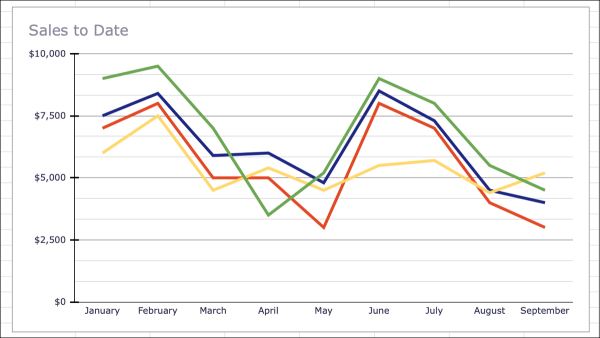
\includegraphics[scale=.5]{figures/line_plot.png}\
    \end{figure}
\end{frame}



\begin{frame}[fragile]
  \noframetitle[0mm]
    \begin{figure}[!htbp]
      \centering
      % can use vspace to adjust figure positioning
      \vspace*{-1.5cm}\caption{Can remove frame title for bigger plots}
      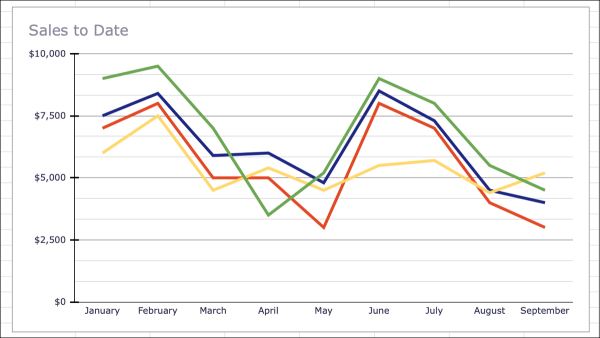
\includegraphics[scale=.7]{figures/line_plot.png}\
    \end{figure}
\end{frame}


\begin{frame}[plain]
  \begin{figure}[!htbp]
    \centering
    \caption{Can use a full blank frame for even bigger plots}
    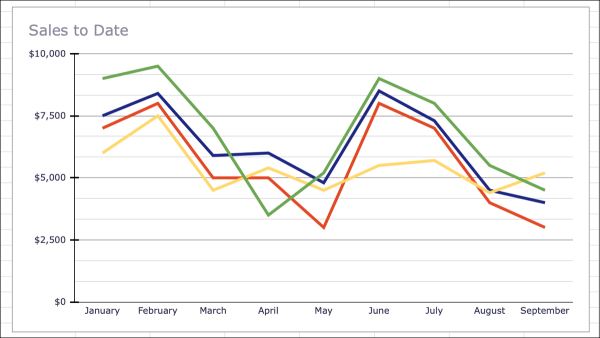
\includegraphics[scale=.8]{figures/line_plot.png}
  \end{figure}
\end{frame}



% ==============================================================
%                         --- Section 4
% ==============================================================
\section{4.0 Conclusion}
\begin{frame}[fragile]
  \frametitle{Blank frame with title}
\end{frame}


\begin{frame}[fragile]
  \noframetitle[0mm]
    Blank frame without title
    \vskip 10mm
\end{frame}



% ==============================================================
%                         --- Bibliography
% ==============================================================

% Can upload bibtex file and save in code/references.bib

\begin{frame}[plain, allowframebreaks]
  \vspace{0.5cm}\center{\Large{\textbf{\textcolor{nclblue}{References}}}}
  \vspace{0.25cm}
  \small
  \bibliographystyle{agsm}
  \bibliography{references}
\end{frame}




% -------------------------------------------------------------
\end{document}
